\section{Evaluation}
\label{sec:evaluation}

\begin{itemize}[itemsep=0pt, topsep=1pt]
\item[\autoref{sec:perf-modeling}] Compared with naive approaches (random and
  gradient-based search), \sysname{} finds a Pareto front that is closer to the
  optimal (\autoref{fig:bo}).
\item[\autoref{sec:runtime}] For all applications, \sysname{} achieves bounded
  service latency across various network conditions (\autoref{fig:end-to-end}).
\end{itemize}

\subsection{Performance Modeling}
\label{sec:perf-modeling}

This section shows that BO can effectively explore the large design space and
come up with a better Pareto-optimal parameter set. We compare \sysname{} with
two baseline profilers: $(i)$ greedy approach as described in
VideoStorm~\cite{zhang2017live}; $(ii)$ random sampling.

Following prior work~\cite{zhang2017live}, several tricks can enhance this
search process. To avoid starting with an expensive configuration and exploring
its neighbors, (which are also likely to be expensive, thus wasting CPU), we
pick k random configurations and start from the one with the highest X(c). We
found that using even k = 3 can successfully avoid starting in an expensive part
of the search space. Second, we cache intermediate results in the query’s DAG
and reuse them in evaluating configura- tions with overlapping knob values. For
each dimen- sion, we could fix the other dimensions and search for the cheapest
configuration possible. This could lead to suboptimal decisions if for example,
because of bad ap- plication configuration a dimension is not fully explored or
there are local minima in the problem space.


Greedy converts MOO into SOO with a parameter $X = \beta$ $A - \beta T$. It
starts with a random configuration $c$ and then picks a neighbor configuration
(by changing the value of a random dimension). If the new configuration $c'$
returns a higher $X$, it updates and iterate form $c'$ again. Otherwise, it
picks a different neighbor $c''$ by changing another dimension. It starts with
three random starting point; it also evaluate a number of random $\beta$.

\autoref{fig:bo} shows that with the same budget (the number of parameters to
evaluate), our profiler can find parameters with better trade-offs between
application accuracy and processing times.

\begin{figure}
  \centering
  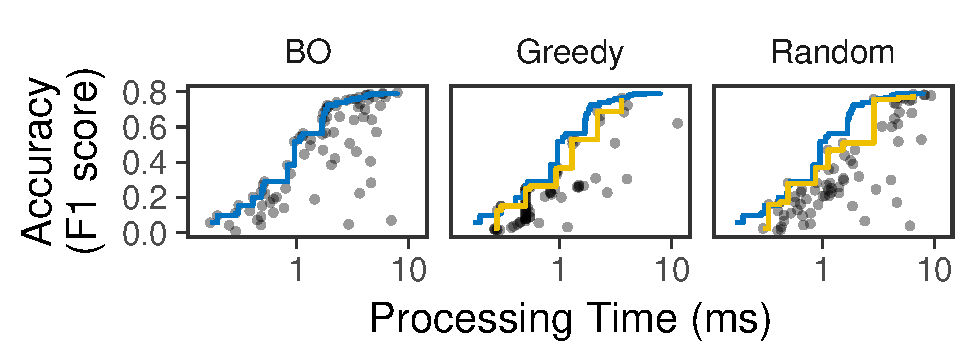
\includegraphics[width=0.85\columnwidth]{figures/profiling.pdf}
  \caption{Using Face as an example, BO evaluates 50 configurations and
    recommends 29 configurations as the Pareto-optimal boundary (the blue
    line). Greedy and Random find sub-optimal Pareto configurations with a
    budget of 80 evaluations (the yellow line in each figure).}
  \label{fig:bo}
\end{figure}

\subsection{Profile Transfer.}

Profile transfer without re-running the entire BO. The ``Pareto-optimal'' is
horizontally stretched/compressed.

\begin{figure}
  \centering
  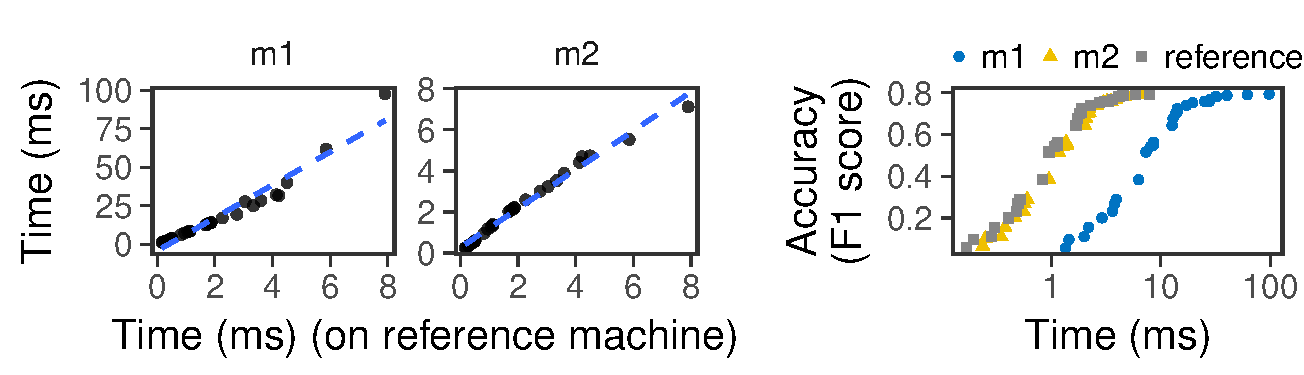
\includegraphics[width=0.9\linewidth]{figures/serving-cross-platform.pdf}
  \caption{(Left) Empirically, processing times follows a linear
    approximation. (Right) Stretched/compressed profile. See paper for
    details.}
\end{figure}

%%% Local Variables:
%%% mode: latex
%%% TeX-master: "../compute"
%%% End:
